\documentclass{standalone}
\usepackage{tikz}
\usetikzlibrary{shapes,arrows,positioning,fit}

\begin{document}
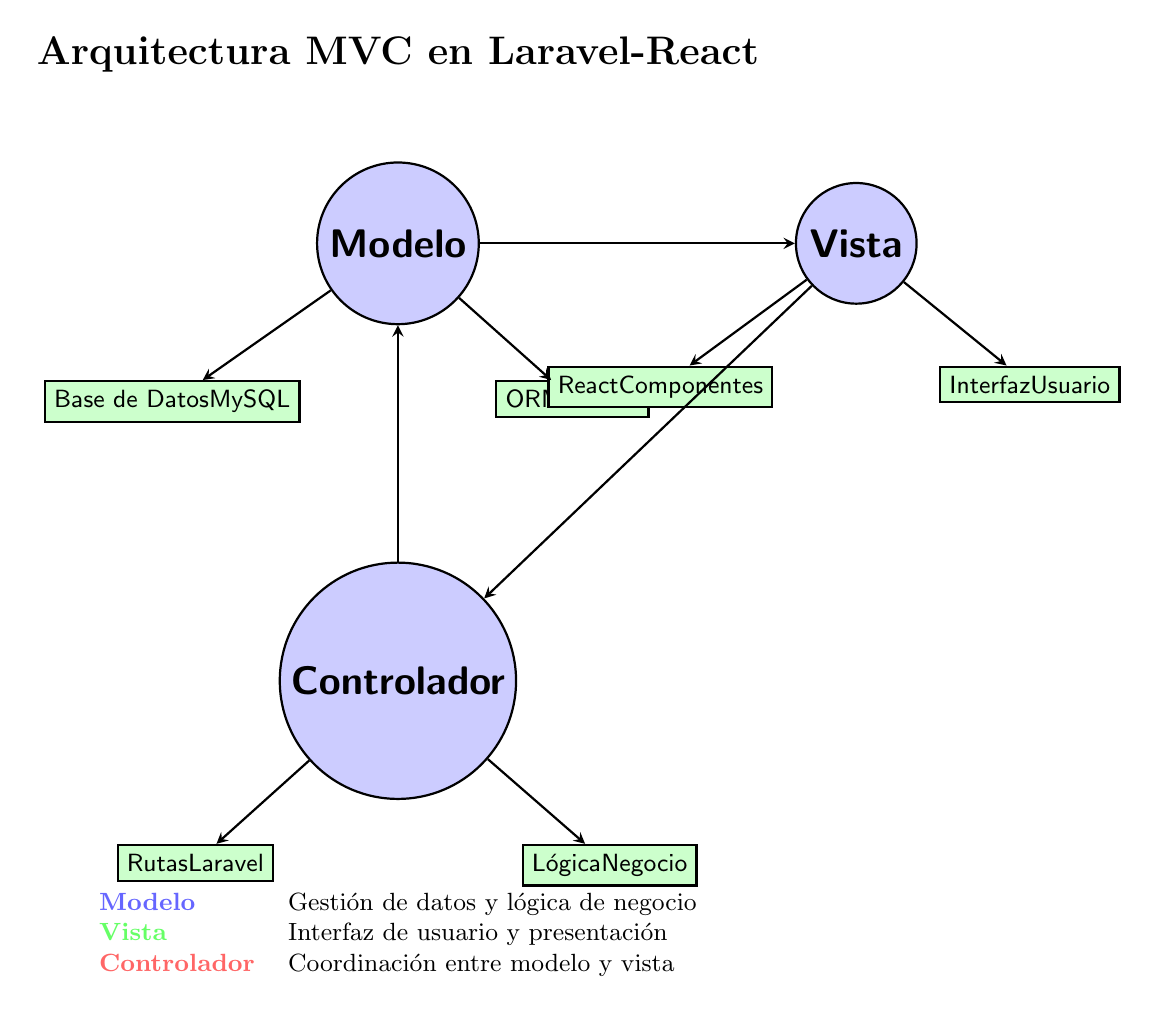
\begin{tikzpicture}[
    node distance=2cm,
    auto,
    thick,
    main node/.style={circle,fill=blue!20,draw,font=\sffamily\Large\bfseries},
    sub node/.style={rectangle,fill=green!20,draw,font=\sffamily\small},
    arrow/.style={->,>=stealth,thick}
]

% Modelo
\node[main node] (model) {Modelo};
\node[sub node, below left=1cm and 0.5cm of model] (database) {Base de Datos\\MySQL};
\node[sub node, below right=1cm and 0.5cm of model] (orm) {ORM\\Laravel};

% Vista
\node[main node, right=4cm of model] (view) {Vista};
\node[sub node, below left=1cm and 0.5cm of view] (react) {React\\Componentes};
\node[sub node, below right=1cm and 0.5cm of view] (ui) {Interfaz\\Usuario};

% Controlador
\node[main node, below=3cm of model] (controller) {Controlador};
\node[sub node, below left=1cm and 0.5cm of controller] (routes) {Rutas\\Laravel};
\node[sub node, below right=1cm and 0.5cm of controller] (logic) {Lógica\\Negocio};

% Conexiones Modelo-Vista-Controlador
\draw[arrow] (model) -- (view);
\draw[arrow] (view) -- (controller);
\draw[arrow] (controller) -- (model);

% Conexiones específicas
\draw[arrow] (model) -- (database);
\draw[arrow] (model) -- (orm);
\draw[arrow] (view) -- (react);
\draw[arrow] (view) -- (ui);
\draw[arrow] (controller) -- (routes);
\draw[arrow] (controller) -- (logic);

% Título
\node[above=1cm of model, font=\Large\bfseries] {Arquitectura MVC en Laravel-React};

% Leyenda
\node[below=1cm of controller, font=\small] {
    \begin{tabular}{ll}
        \textcolor{blue!60}{\textbf{Modelo}} & Gestión de datos y lógica de negocio \\
        \textcolor{green!60}{\textbf{Vista}} & Interfaz de usuario y presentación \\
        \textcolor{red!60}{\textbf{Controlador}} & Coordinación entre modelo y vista
    \end{tabular}
};

\end{tikzpicture}
\end{document}
